%%%%%%%%%%%%%%%%%%%%%%%%%%%%%%%%%%%%%%%%%%%%%%%%%%%%%%%%%%
%% SLIDE 3: THE PROBLEM — PRICE TAG INEFFICIENCY
%% CORE PITCH
%%%%%%%%%%%%%%%%%%%%%%%%%%%%%%%%%%%%%%%%%%%%%%%%%%%%%%%%%%

\begin{frame}
    \begin{tikzpicture}[remember picture,overlay]
        \fill[PrimaryGoldLight, opacity=0.08] ([xshift=0cm,yshift=0cm]current page.center) circle (4cm);
        \node[anchor=north west, text=FundoQuestion, font=\bfseries\tamanhoQuestion\selectfont]
            at ([xshift=0.8cm,yshift=-0.8cm]current page.north west) {What is wrong with the physical price tag?};
        \node[anchor=north west, text width=.80\paperwidth, align=left, text=FundoKeyMessage, font=\tamanhoKeyMessage\selectfont]
            at ([xshift=0.8cm,yshift=-1.6cm]current page.north west) {
            It is static, costly to update, and can only tell customers the price—not help them shop.
        };
    \end{tikzpicture}

    \vspace{0.3cm}
    \begin{center}
        {\Huge\bfseries\textcolor{PrimaryBlue}{The Price Tag is a Relic}}
        \vspace{0.05cm}
    \end{center}

    \vspace{0.1cm}
    \begin{columns}[T]
        \column{0.35\textwidth}
        \begin{center}
            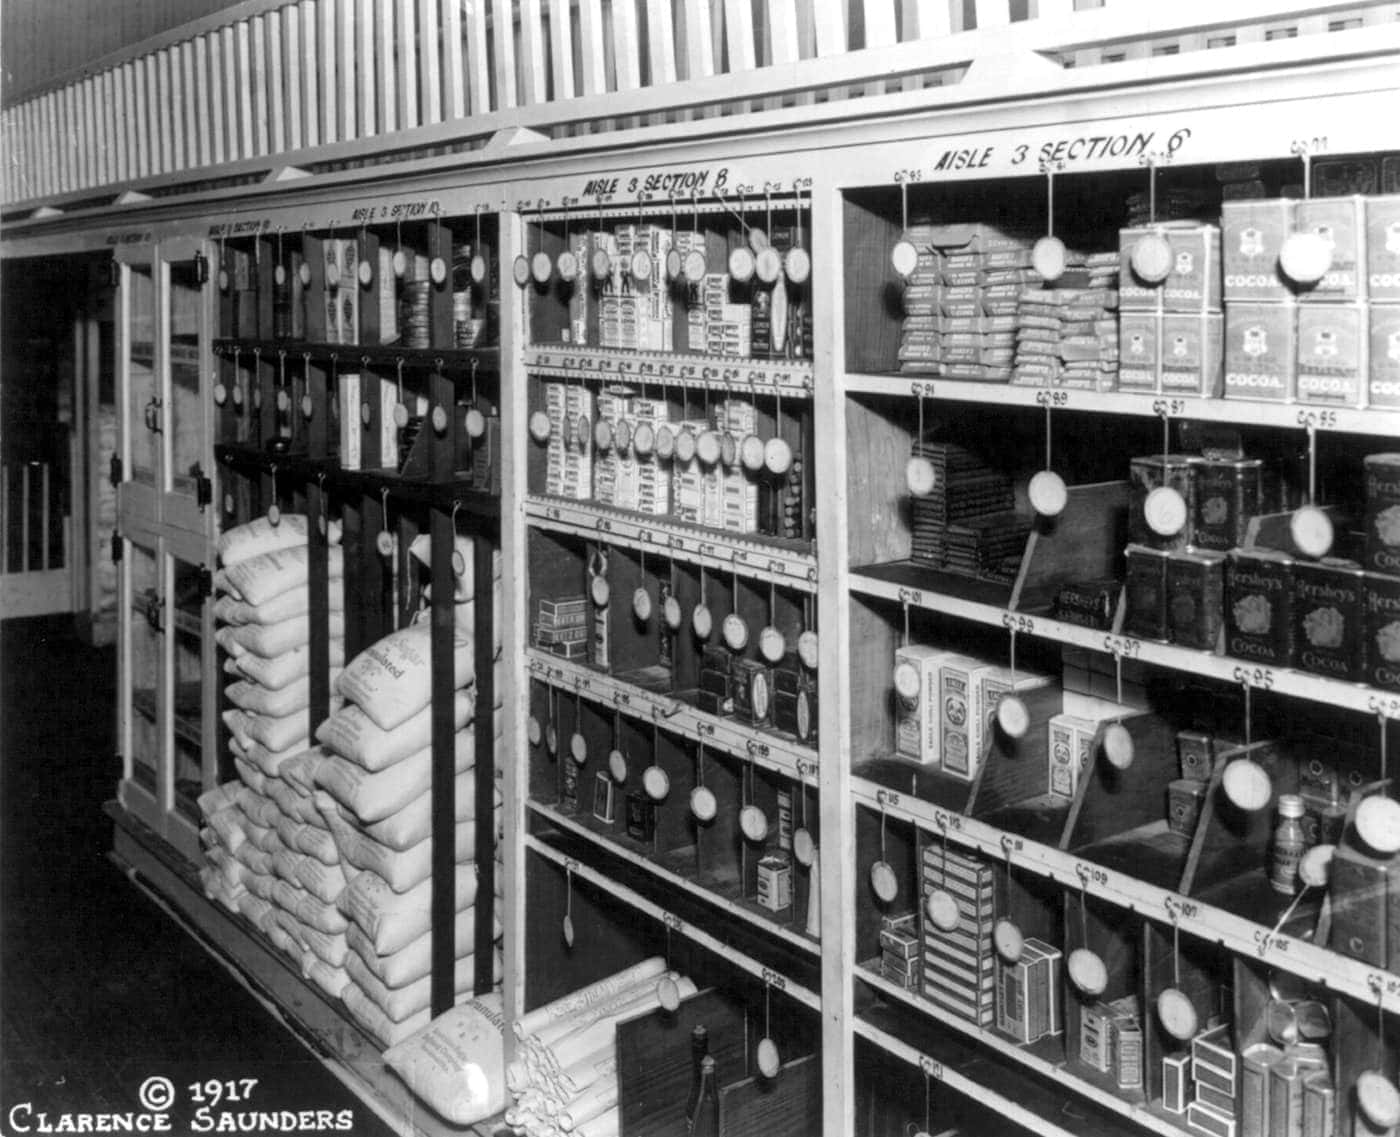
\includegraphics[width=4.8cm, height=6.0cm, keepaspectratio]{Images/Antique-Piggly-Wiggly-grocery-store-from-1917-6.jpg}
            \vspace{0.2cm}
            \source{Piggly-Wiggly, 1917}
        \end{center}
        
        \column{0.60\textwidth}
        \begin{center}
            \begin{tikzpicture}[
                node distance=0.15cm,
                issue/.style={
                    draw=PrimaryRed!30,
                    rounded corners=4pt,
                    minimum width=6.0cm,
                    minimum height=0.6cm,
                    align=left,
                    fill=white,
                    line width=0.8pt,
                    font=\footnotesize
                }
            ]
                \node[issue, fill=RedCard, draw=PrimaryRed] (i1) {
                    \textcolor{PrimaryRed}{\textbf{$\times$}} \textcolor{BodyText}{Costly to print and manage}
                };
                \node[issue, below=0.15cm of i1, fill=RedCard, draw=PrimaryRed] (i2) {
                    \textcolor{PrimaryRed}{\textbf{$\times$}} \textcolor{BodyText}{Static — cannot adapt to demand}
                };
                \node[issue, below=0.15cm of i2, fill=RedCard, draw=PrimaryRed] (i3) {
                    \textcolor{PrimaryRed}{\textbf{$\times$}} \textcolor{BodyText}{One-way — no customer interaction}
                };
                \node[issue, below=0.15cm of i3, fill=RedCard, draw=PrimaryRed] (i4) {
                    \textcolor{PrimaryRed}{\textbf{$\times$}} \textcolor{BodyText}{No data capture, no intelligence}
                };
                \node[issue, below=0.15cm of i4, fill=RedCard, draw=PrimaryRed] (i5) {
                    \textcolor{PrimaryRed}{\textbf{$\times$}} \textcolor{BodyText}{Manual errors and inconsistencies}
                };
            \end{tikzpicture}
        \end{center}
    \end{columns}

    \vspace{-0.2cm}
    \begin{center}
        \begin{tikzpicture}
            \node[draw=PrimaryBlue, fill=BlueCard, rounded corners=6pt, 
                  minimum width=10.5cm, minimum height=0.6cm, 
                  align=center, line width=1.5pt, font=\small] {
                \textcolor{PrimaryBlue}{A 20th-century solution for a 21st-century problem.}
            };
        \end{tikzpicture}
    \end{center}
\end{frame}